\chapter{Ovládání přes mobilní telfon}
%Nemám nejmenší tušení co jsem psát, protože o té webovce nic, ale vůůůůůbec nic nevím

\section{Esp32-RBGridUI-Designer} 
Pro vytvoření ovládacího prostředí na mobilním telefonu, jsem použila {RBGridUI-Designer} \cite{RBGridUI-Designer}, což je prostředí vyvinuté přímo Robotárnou \cite{robotarna} pro práci s LED a jejich ovládání přes mobilní telefon.

Webová stránka {\em Esp32-RBGridUI-Designer} má toto rozložení: 

\begin{figure}[htbp]
	\centering
	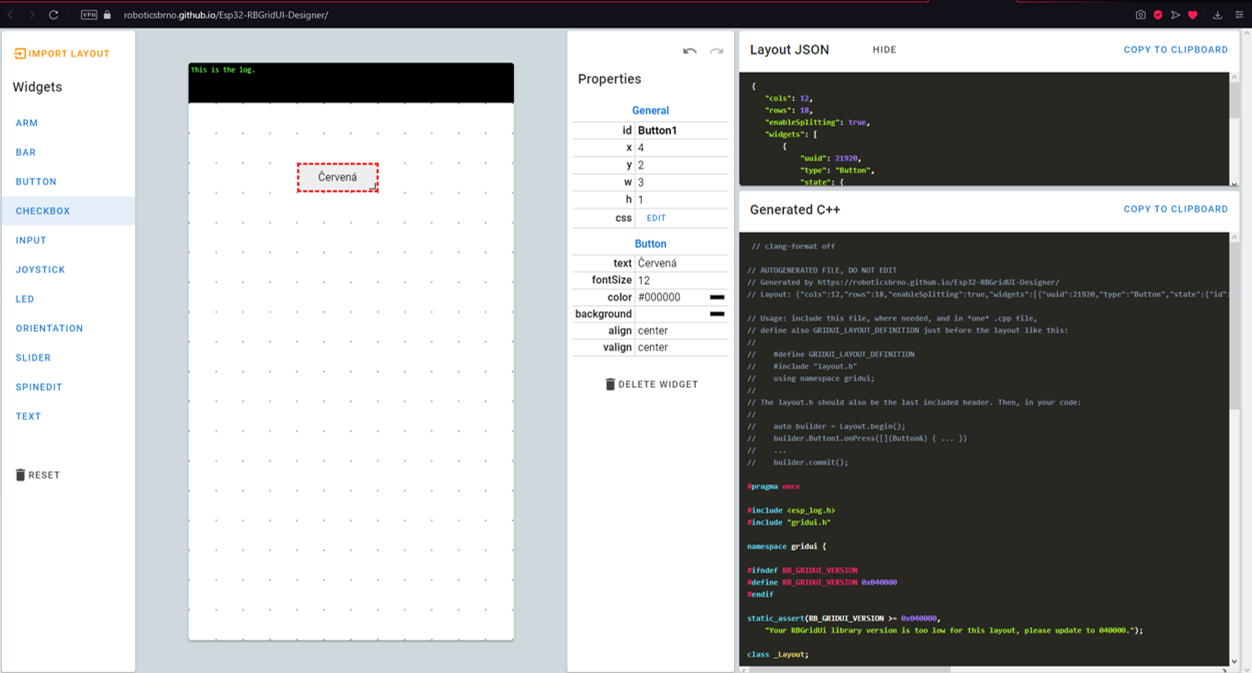
\includegraphics[width=1\textwidth]{img/Esp32-RBGridUI-Designer.png}
	\caption{Prostředí stránky {\em Esp32-RBGridUI-Designer}}
	%	\label{fig:install-sdk-3}
\end{figure}

\begin{enumerate}
	\item Postraní lišta, při kliknutí na jakoukoliv komponentu, je uživatel schopen danou kamponentu přetáhnout na manipulační plochu. 
	\item Manipulační plocha, na kterou se umisťují komponenty z postranní lišty. Nastavuje se tu jejich poloha a umístění. Manipulační plocha určuje vzhled řídící plochy v aplikaci v mobilním telefonu při napojení na daný Wifi modul. 
	\item  Tuto tabulku pro práci s ESP32-DevKitC potřebovat nebudeme.
	\item  Soubor Layout, který je potřeba stáhnout a nahrát do stejné složky jako máme hlavní program. Tento soubor nese informace toho, jakým způsobem jsme nanesli komponenty na manipulační plochu.
	\item Bližší specifikace, určující umístění, barvu, a název tlačítka, které bylo vytvořeno na~manipulační ploše. Tyto informace je možné zde i předělávat a upravovat.
	\item Tlačítko Reset které vymaže veškeré komponenty z Manipulační plochy a tím pádem i z Layoutu.
\end{enumerate}


% {\em Esp32-RBGridUI-Designer} je propojený s aplikací {\em RBControler,} \cite{RBControler}

\section{Vytvoření tlačítek}
Abych mohla barvy na LED ovládat a libovolně mezi nimi přepínat, rozhodla jsem se v~{\em RBGridUI-Designeru} vytvořit 5 tlačítek: co tlačítko, to jeden mód a tlačítko na vypnutí světel. Tlačítka jsem si pojmenovala tak, abych se v barvách vyznala a trochu jsem si i~pohrála s barvami tlačítek. Poté mi už jen stačilo zkopírovat soubor layout do samostatného textového souboru, pozměnit příponu souboru z {\em .txt} na {\em .hpp} a umístit ho do stejné složky, jako hlavní program.
%todo Otázka --> obrázek z FreeComanderu?

%\begin{figure}[htbp]
%	\centering
%	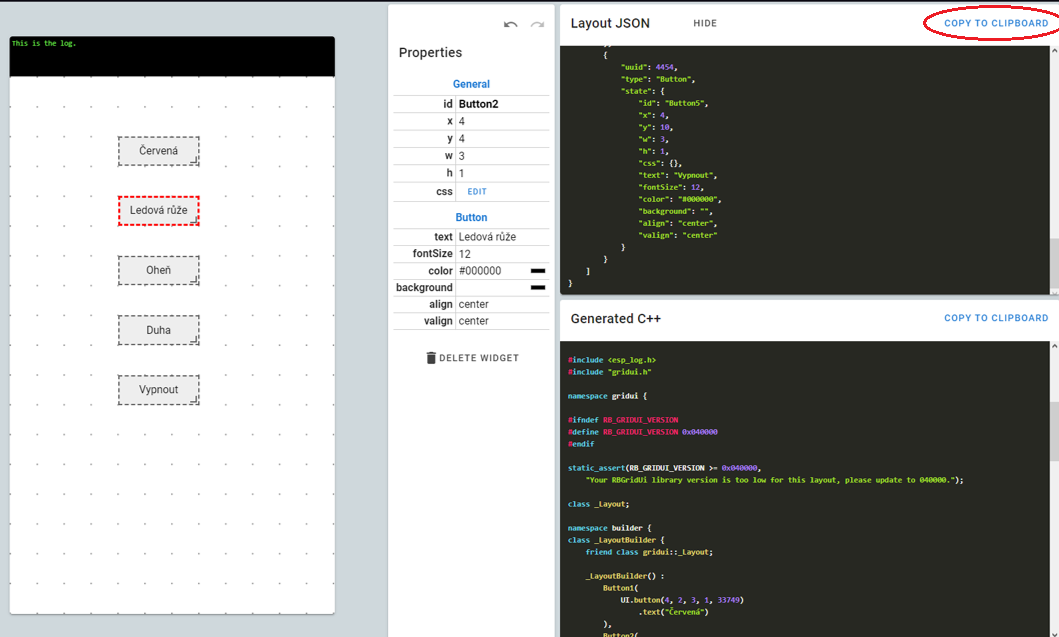
\includegraphics[width=0.8\textwidth]{img/Esp32-RBGridUI-Designer - Tlačítka.png}
%	\caption{Tlačítka}
	%	\label{fig:install-sdk-3}
%\end{figure}
%sooooo messy...

~
%todo Nebere mi to odkazy na github
\section{Hlavní Program} 
Nyní nastal čas spojit veškeré programy jednotlivých barevných módů do jediného a  \href{https://github.com/Nemesis-Rain/Supplements-/tree/main/Final-program}{finálního programu}, který budeme používat a bude naším konečným výsledkem po programovací stránce. 
Naštěstí jsem část finální program nemusela tvořit úplně z ničeho a využila jsem části jednoho \href{https://github.com/Nemesis-Rain/Supplements-/tree/main/Original-program-layout}{darovaného programu}.
 Tyto části se zabývaly propojením ESP32-DevKitC s~mobilním telefonem pomocí Wifi modulu. Stačilo tedy barevné módy do programu šikovně zapracovat a vymazat nepotřebné kusy kódu.

%todo Otázka --> Mám problémy s proklikávacími odkazy na github


Následující program ukazuje jen části Hlavního programu. 

Funkce {\em void Setup()} ukazuje nastavení jména a hesla na Wifi, propojení s {\em Layout.hpp} ve stejné složce a pak definování a funkci jednotlivých tlačítek, které jsme si nastavili už~předtím v {\em RBGridUI-Designeru.}

Funkce {\em void Loop()} dokončuje ukázku definování tlačítek, která je provedená pomocí příkazu {\em switch.}


\lstinputlisting{Code/new-program - Setup.cpp}

\lstinputlisting{Code/new-program - Loop.cpp}

\newpage

\section{Propojení mobilního telefonu a ESP32-DevkitC a kontrola funkčnosti}
Na Google play na mobilním telefonu jsem si našla aplikaci jménem \href{https://play.google.com/store/apps/details?id=com.tassadar.rbcontroller}{RB Controler}, také vytvořená pod vedením \href{https://helceletka.cz/robotarna/}{Robotárny}. Aplikaci jsem si nainstalovala a spustila.

Poté jsem zapojila ESP32-DevkitC, ověřila jsem si, že je v něm nahraný Hlavní program a připojila jsem se na Wifi jménem LEDLED. 

Po aktualizaci aplikace se mi na obrazovce objevilo:

%Ukol-J --> Zde bude screenshot obrazovky mého mobilu.

\begin{figure}[htbp]
	\centering
	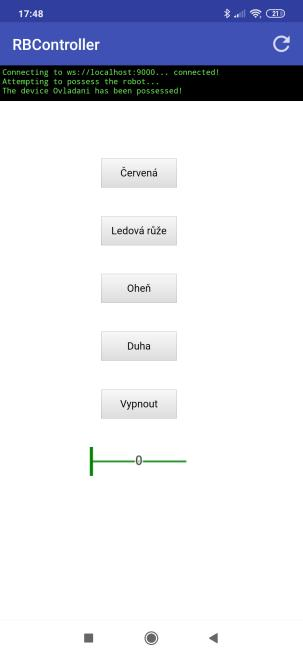
\includegraphics[width=0.25\textwidth]{img/Screenshot- rbcontroller.jpg}
	\caption{Aplikace RBControler - ovládací panel}
	%	\label{fig:install-sdk-3}
\end{figure}



Teď už jenom chtělo vyzkoušet, jak moc je daný program kompatibilní a funkční.
 
%todo odkaz na video? +++ VIDEO


\section{Vyměnění LED pásků}

Jelikož mi LED blikaly přesně tak, jak jsem zamýšlela, rozhodla jsem se provést poslední krok, a to výměnu pevného LED pásku za pásek ohebný, který jsem zmínila předtím už v~první kapitole. 

\begin{figure}[htbp]
	\centering
	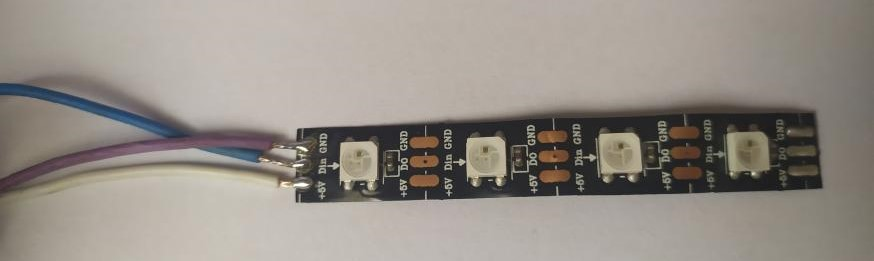
\includegraphics[width=0.5\textwidth]{img/4Led2.jpg}
	\caption{Zapájený ohebný LED pásek}
	%	\label{fig:install-sdk-3}
\end{figure}

Nebylo to nic  těžkého. Tři krátké dráty jsem připájela na tři předem připravené kontakty: GND, DIN a 5V. Na druhé konce drátů jsem přidělala pinheady, které jsem připojila k~\textit{ESP32-DevkitC}. Jako vstupní pin jsem znovu zvolila pin 21.

Aby tento pásek fungoval, musela jsem v programu pozměnit proměnnou {\em LED\_COUNT} z 8 na 4, protože ohebný pásek na rozdíl od testovacího měl pouze 4 LED. 

\lstinputlisting{Code/Novy-zacatek-programu.cpp}


